\documentclass[10pt]{article}
\usepackage[margin=0.5in,top=0.4in,bottom=0.35in]{geometry}
\usepackage{graphicx}
\usepackage{caption}
\usepackage{subcaption}
\usepackage{float}
\usepackage{xcolor}
\usepackage[hidelinks]{hyperref}

\setlength{\parskip}{2pt}
\setlength{\parindent}{0pt}
\setlength{\abovecaptionskip}{4pt}
\setlength{\belowcaptionskip}{2pt}
\captionsetup{font=small}

\pagestyle{empty}

\begin{document}

\begin{center}
{\Large\bfseries Autoreason --- Experimental Results}\\[2pt]
{\small Nous Research \quad $\cdot$ \quad \url{https://github.com/NousResearch/autoreason}}
\end{center}

\vspace{2pt}

\begin{figure}[H]
\centering
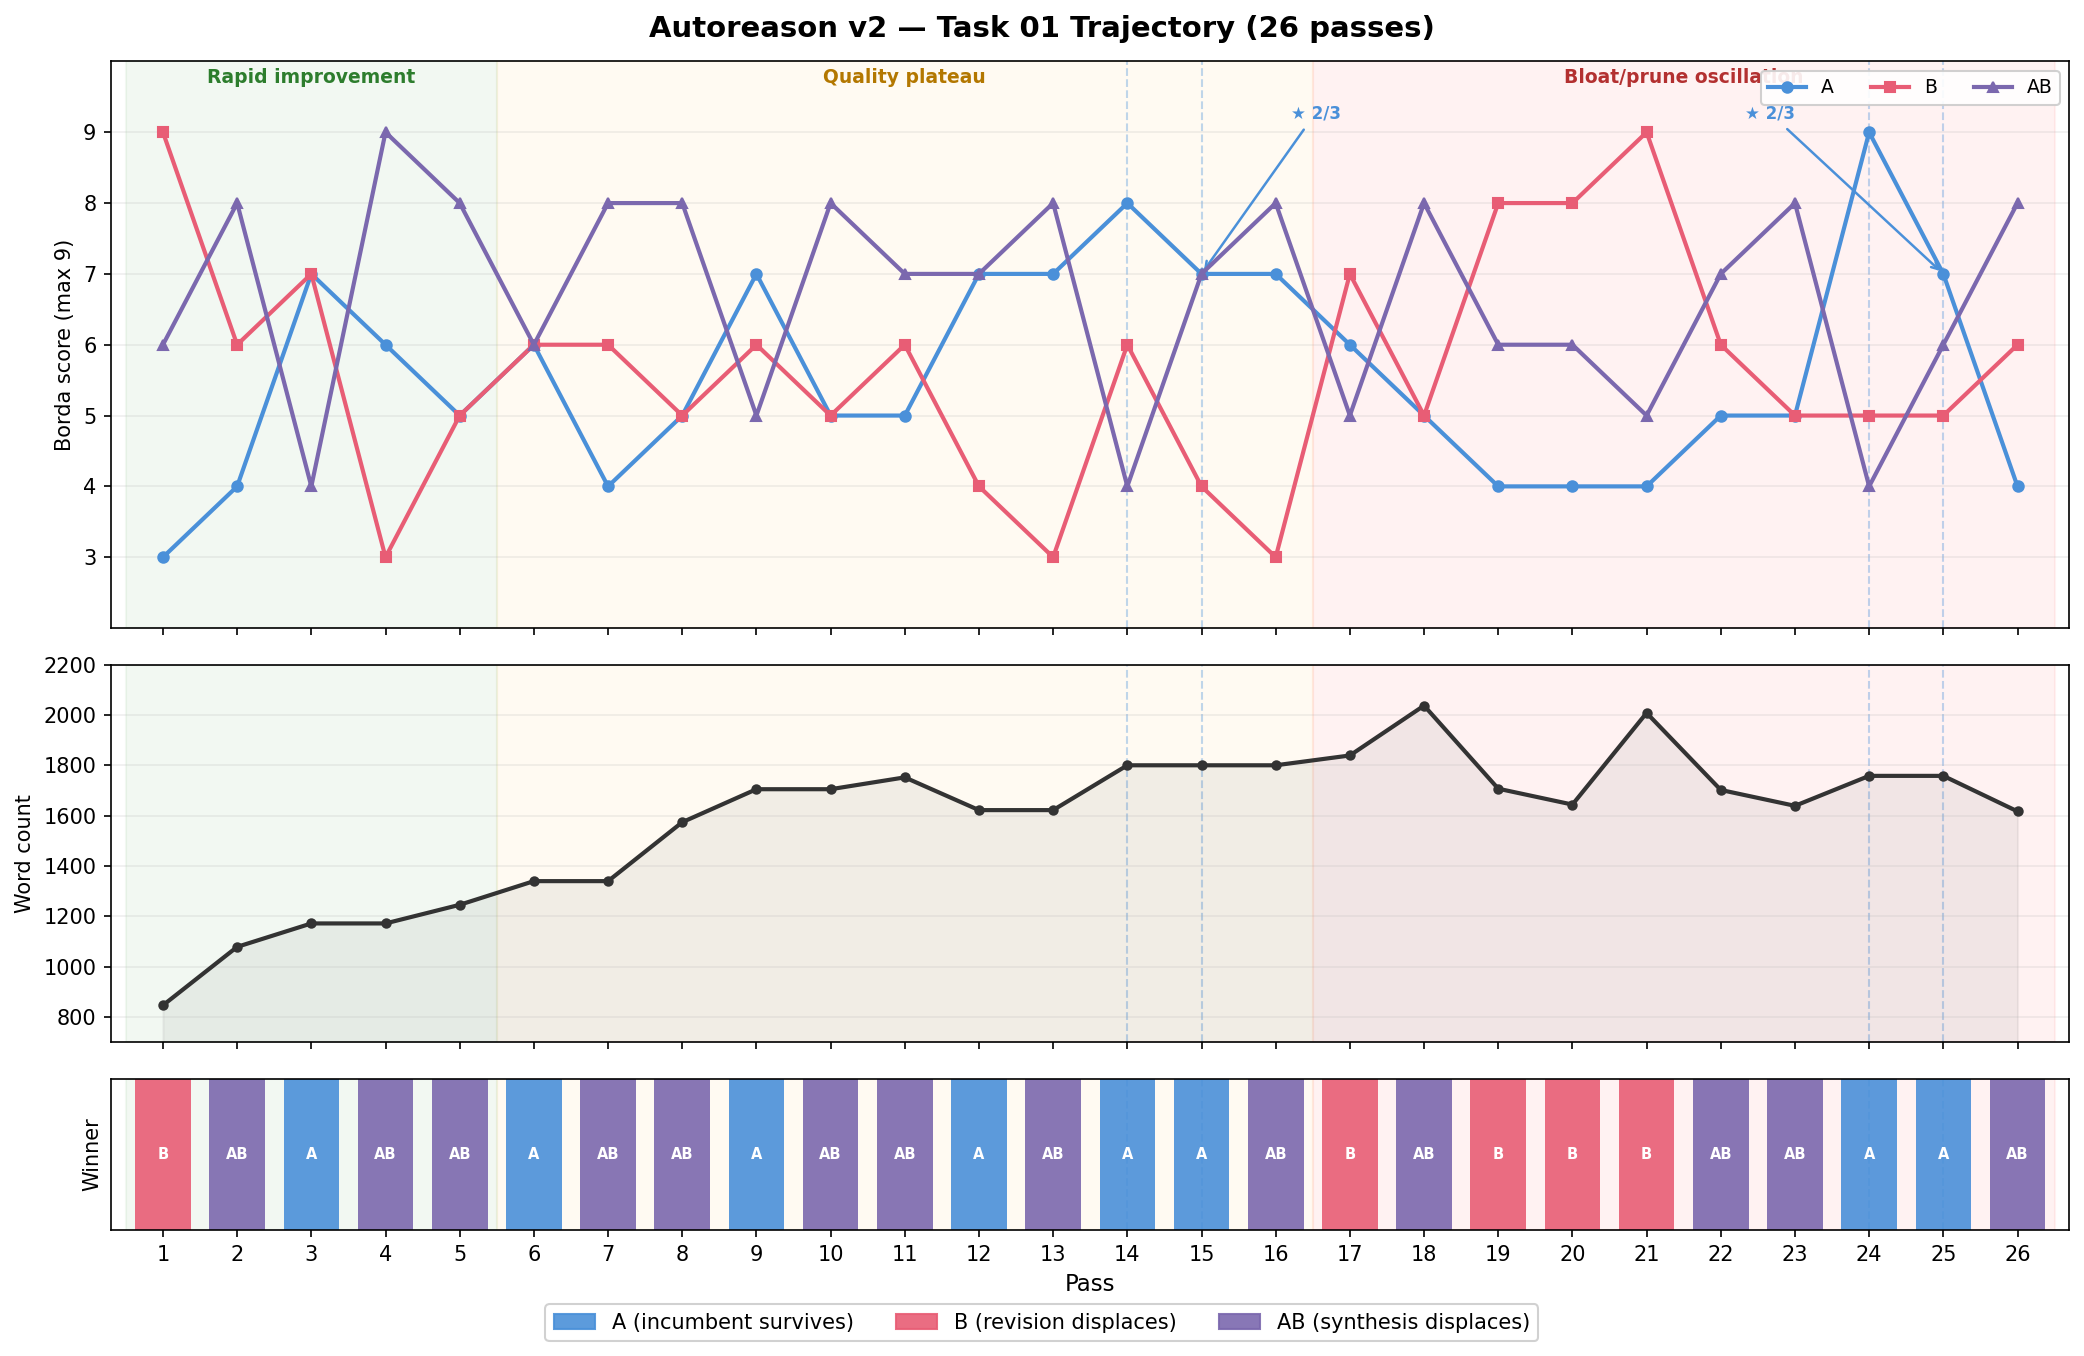
\includegraphics[width=0.95\textwidth,height=3.8cm,keepaspectratio]{fig_trajectory.png}
\caption{\textbf{Autoreason v2 trajectory (26 passes).} Top: Borda scores per pass. Middle: word count showing bloat/prune oscillation. Bottom: winner. Dashed lines mark 2-consecutive-A-win points.}
\end{figure}

\vspace{-2pt}

\begin{figure}[H]
\centering
\begin{subfigure}[t]{0.48\textwidth}
\centering
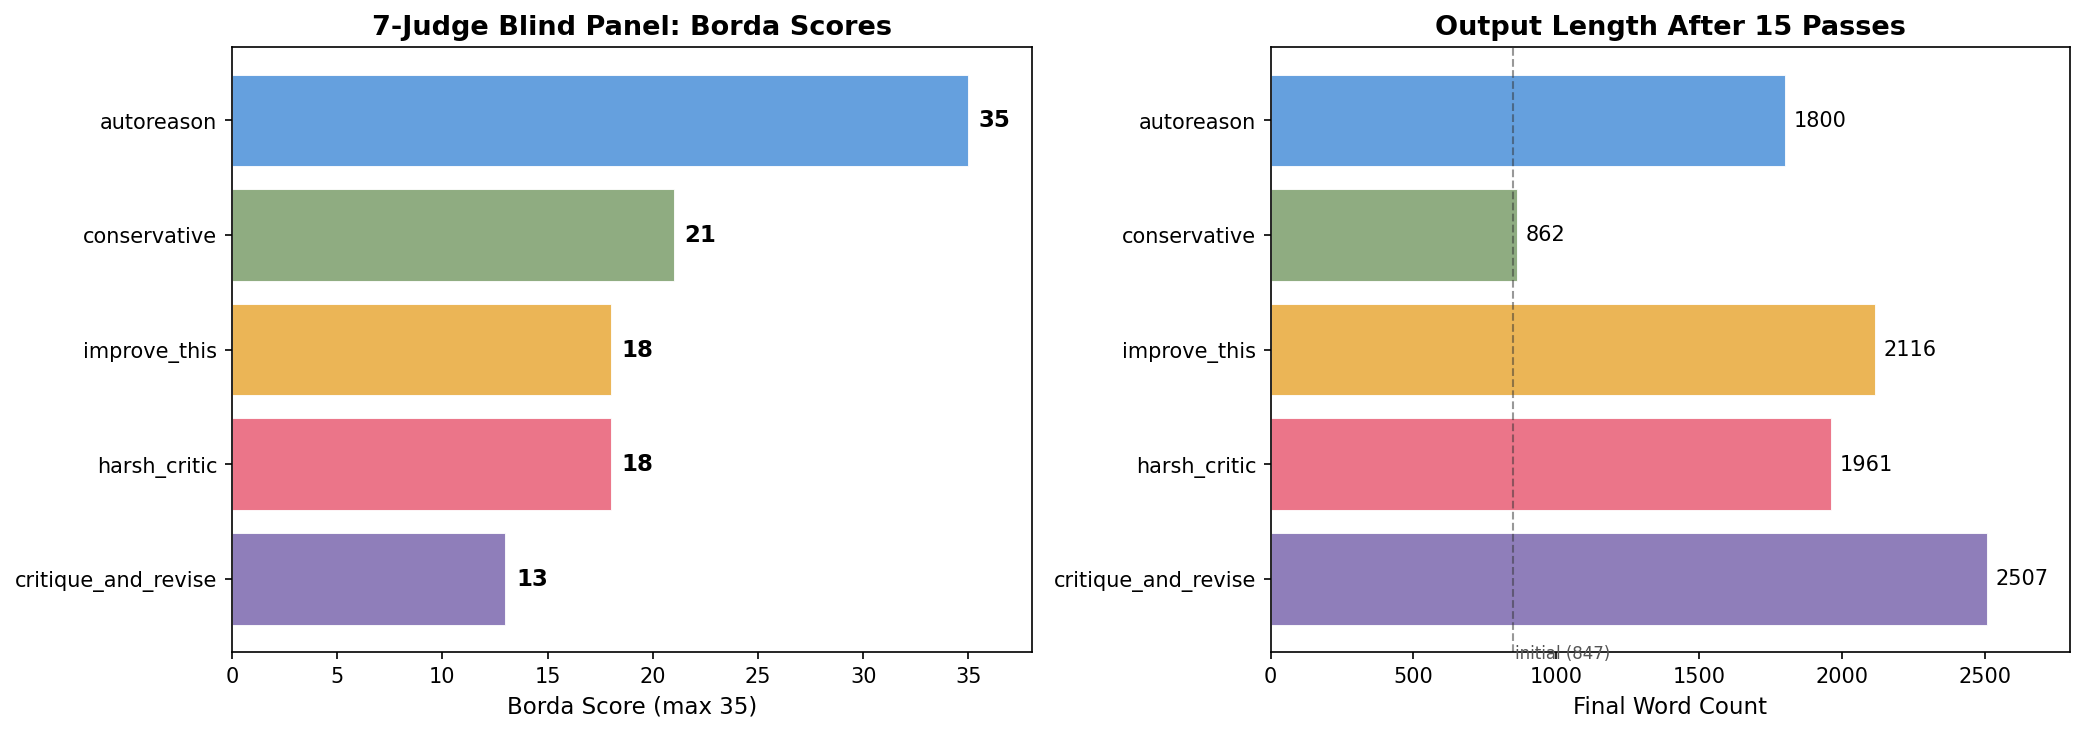
\includegraphics[width=\textwidth,height=3.5cm,keepaspectratio]{fig_baseline.png}
\caption{\textbf{7-judge blind panel.} Borda scores (left) and word counts (right). Autoreason: 35/35, 7/7 first place. Conservative outranks all iterative baselines.}
\end{subfigure}
\hfill
\begin{subfigure}[t]{0.48\textwidth}
\centering
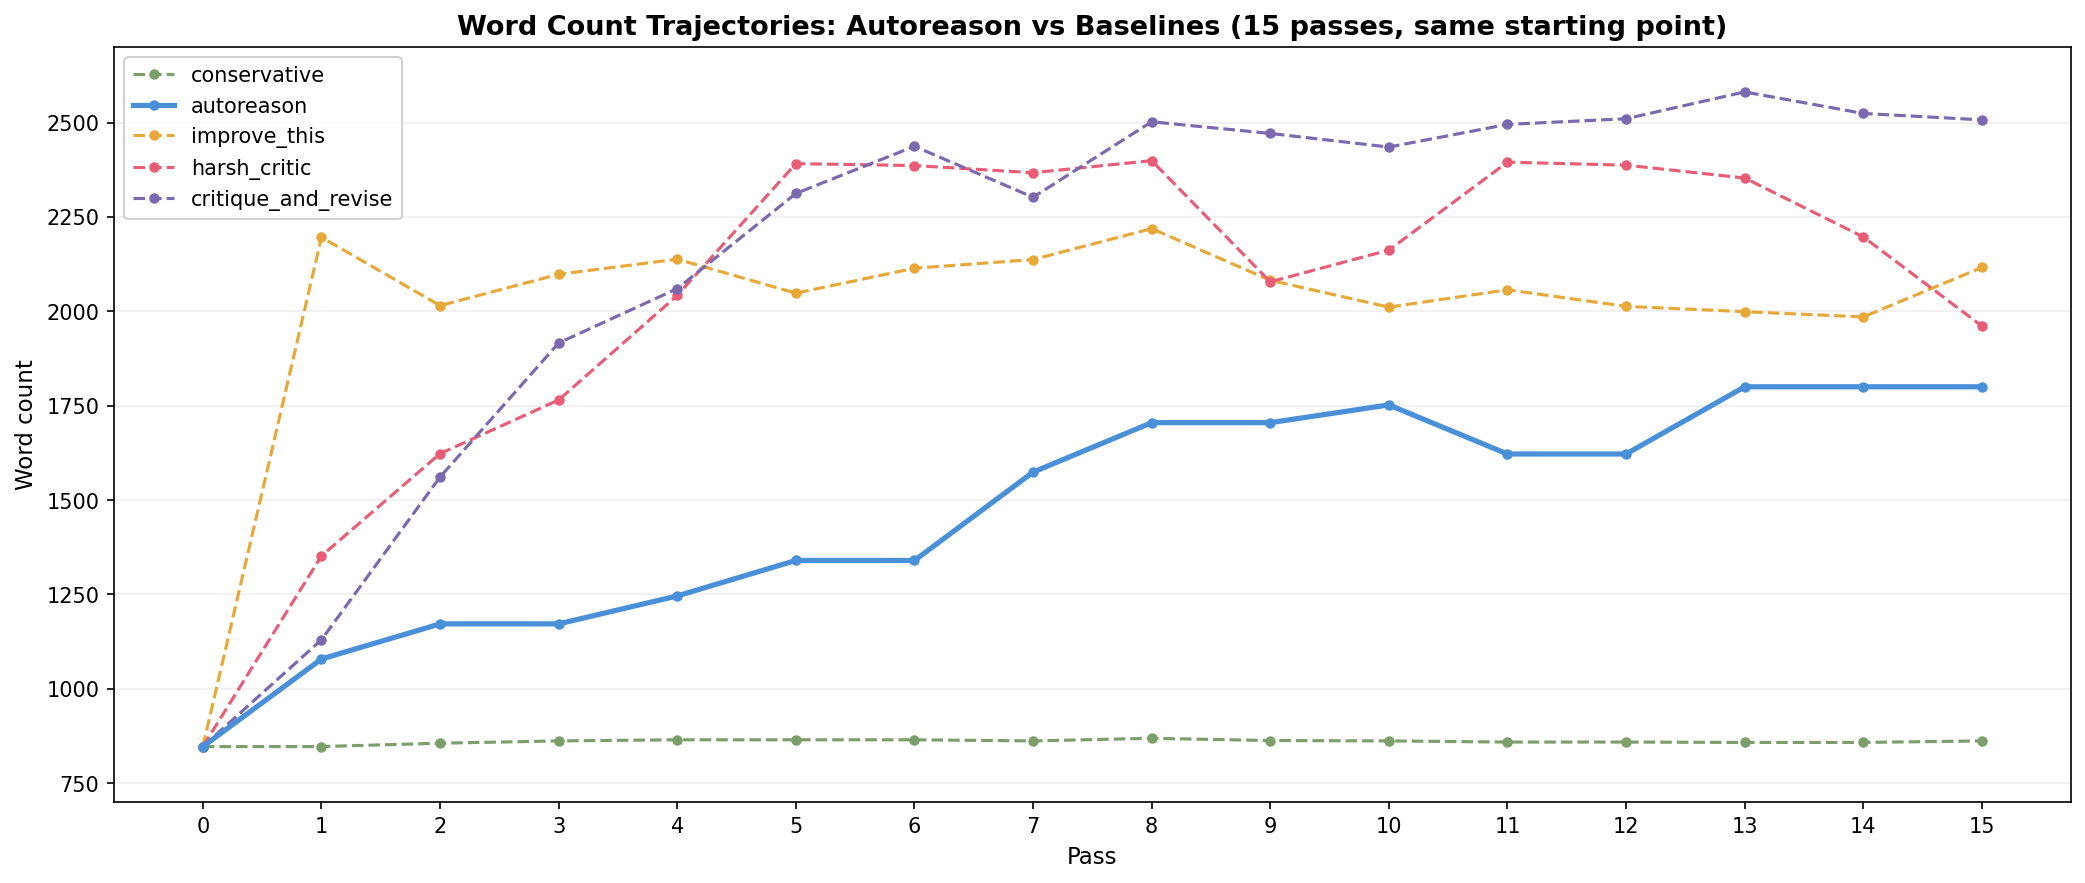
\includegraphics[width=\textwidth,height=3.5cm,keepaspectratio]{fig_wordcount.png}
\caption{\textbf{Word count trajectories.} Conservative flatlines, autoreason stabilizes, iterative baselines bloat. Critique-and-revise bloats most, scores worst.}
\end{subfigure}
\caption{\textbf{Baseline comparison.} Same start (847 words), same model, 15 passes. Judges see task, initial output, and all 5 finals (randomized labels).}
\end{figure}

\vspace{-2pt}

\begin{figure}[H]
\centering
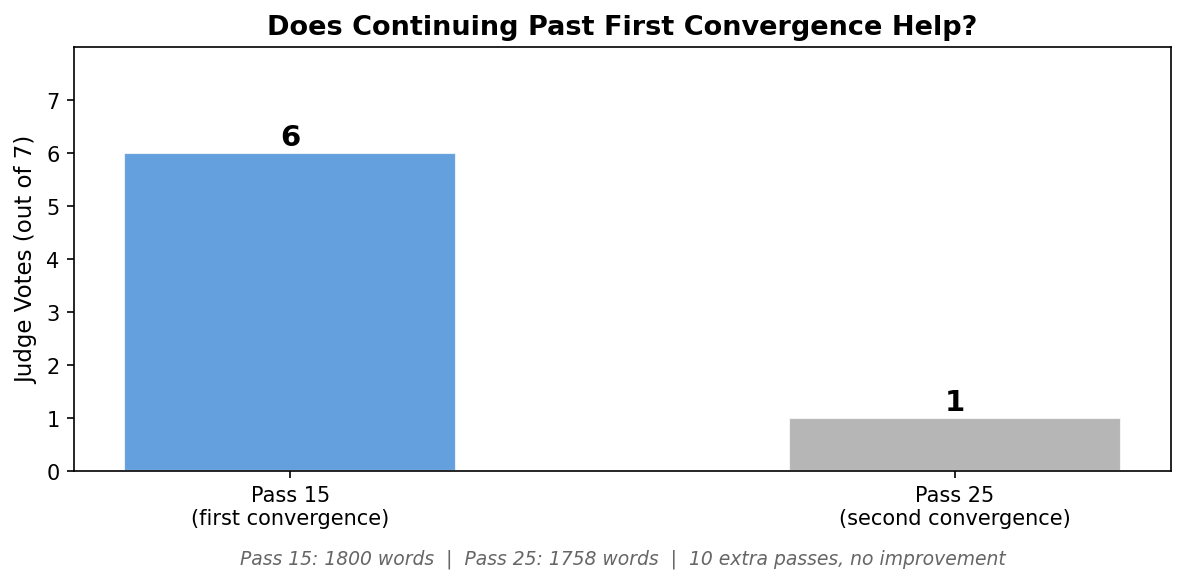
\includegraphics[width=0.48\textwidth,height=3.2cm,keepaspectratio]{fig_convergence.png}
\caption{\textbf{Does continuing past first convergence help?} Pass 15 vs pass 25, 7-judge blind panel: 6--1 for pass 15. First convergence is the quality ceiling.}
\end{figure}

\end{document}
